\documentclass[12pt]{scrartcl}
\usepackage[margin=1.2in]{geometry}
\usepackage[french]{babel} % choix de la langue : anglais par défaut
\usepackage[utf8]{inputenc} % choix de l'encodage des caractères : utile pour les accents
\usepackage[T1]{fontenc} 
\usepackage{fancyhdr}
\usepackage{setspace}
\usepackage{enumitem}
\usepackage{subfig}
\onehalfspacing
%%%%%%%%%%%%%%%%%%%%%%%%%%%%%%%%%%%%%%%%%%%%%%%%%%%%
% Grammaire :
\usepackage{listings}

\lstset{
  xleftmargin=3em,
  literate={->}{$\rightarrow$}{2},
  literate={eps}{$\varepsilon$}{3},
}
%%%%%%%%%%%%%%%%%%%%%%%%%%%%%%%%%%%%%%%%%%%%%%%%%%%%
% Math : les packages classiques : 
\usepackage{amsmath} 
\usepackage{amssymb} 

%%%%%%%%%%%%%%%%%%%%%%%%%%%%%%%%%%%%%%%%%%%%%%%%%%%%
% Algo : 
\usepackage[french]{algorithm2e} 

%%%%%%%%%%%%%%%%%%%%%%%%%%%%%%%%%%%%%%%%%%%%%%%%%%%%
% graphique
\usepackage{graphicx} 
\graphicspath{ {./img/} }

\begin{document}
%%%%%%%%%%%%%%%%%%%%%%%%%%%%%%%%%%%%%%%%%%%%%%%%%%%%%%%%%%%
% DOCUMENT
\pagestyle{fancy}
\rhead{  }
\lfoot{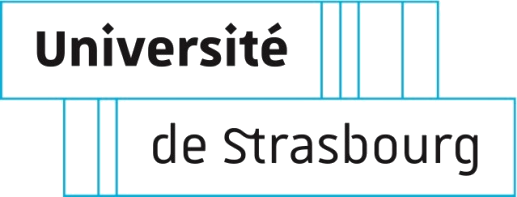
\includegraphics[scale=0.2]{logounistra}}

\title{%
Simulation d'exécution de programmes parallèles\\
\large } 

\subtitle{ Travail d'étude et de recherche. \\Rapport. }
\author{Olga Pigareva\\
M1 SIL} % optionnel

% \date est optionnel : par défaut, date du jour de compilation
% \date{aujourd'hui} % date fixe
% \date{} % pas de date




\maketitle

\newpage

%%%%%%%%%%%%%%%%%%%%%%%%%%%%%%%%%%%%%%%%%%%%%%%%%%%%
\tableofcontents % facultatif

\newpage % permet de changer de page
%%%%%%%%%%%%%%%%%%%%%%%%%%%%%%%%%%%%%%%%%%%%%%%%%%%%
\section{La présentation de la problématique dans son contexte}

\subsection{Introduction}
Le sujet de mon travail d'étude et de recherche aborde un domaine d'actualité dans le monde numérique, la programmation parallèle.
La parallélisation de tâches et de processus permet d'augmenter la performance et faire l'exécution d'un programme beaucoup plus rapide. 
C'est pourquoi la programmation parallèle reste un sujet très actuel, même si elle était inventée il y a déjà plusieurs années.\\

La programmation parallèle comprend la résolution d'un problème simultanément par plusieurs processus.
Cela implique l'utilisation d'une seule ressource par plusieurs processus, ce qui nécessite une synchronisation.
De son côté, la synchronisation peut amener à un interblocage qui peut avoir les conséquences indésirables (catastrophiques) pour un programme. \\
Mon travail fait partie d'une recherche visant à caractériser ces interblocages.\\
Dans les parties suivantes, j'expliquerai ce que signifient ces termes.   
%Cela implique Mais quand il y a plusieurs processus qui utilisent la même ressource, l'interblocage peut apparaître. Par exemple, si on a un processus attent un autre processus, qui de sa part attends le première processus. Le programme restera bloqué qui implique plusieurs problèmes. 
%C'est pourquoi on cherche d'éviter et de reconnaître un interblocage le plus tôt possible.
%%%%%%%%%%%%%%%%%%%%%%%%%%%%%%%%%%%%%%%%%%%%%%%%%%%%
\subsection{Programmes parallèles}

Les programmes parallèles permettent de créer les activités qui peuvent exécuter les instructions indépendamment. 
Souvent ces activités ont besoin d'acceder aux mêmes ressources. 
Pour ne pas avoir des résultats imprévus lors de modification de données par les processus différents, les ressources sont synchronisées. 
Cela veut dire que les processus peuvent acceder aux données chacun à son tour. 
Pour attendre la libération de données ou la fin d'instructions d'un processus, un programme parallèle utilise les horloges qui sont les barrières de synchronisation.
\newpage
%%%%%%%%%%%%%%%%%%%%%%%%%%%%%%%%%%%%%%%%%%%%%%%%%%%%
\subsection{Interblocage}

Le problème d'interblocage apparaît quand chaque processus attend un autre pour se terminer et finalement aucun peut acceder à la ressource.
Par conséquent, le programme reste bloqué.\\

Par exemple, sur la Figure 1, le processus P1 attend la fin de processus P2 pour acceder à R1. Et P2, de son côté, attend la fin de P1 pour acceder à R2. Tous les deux processus restent bloqués.\\

\begin{figure}[h]
  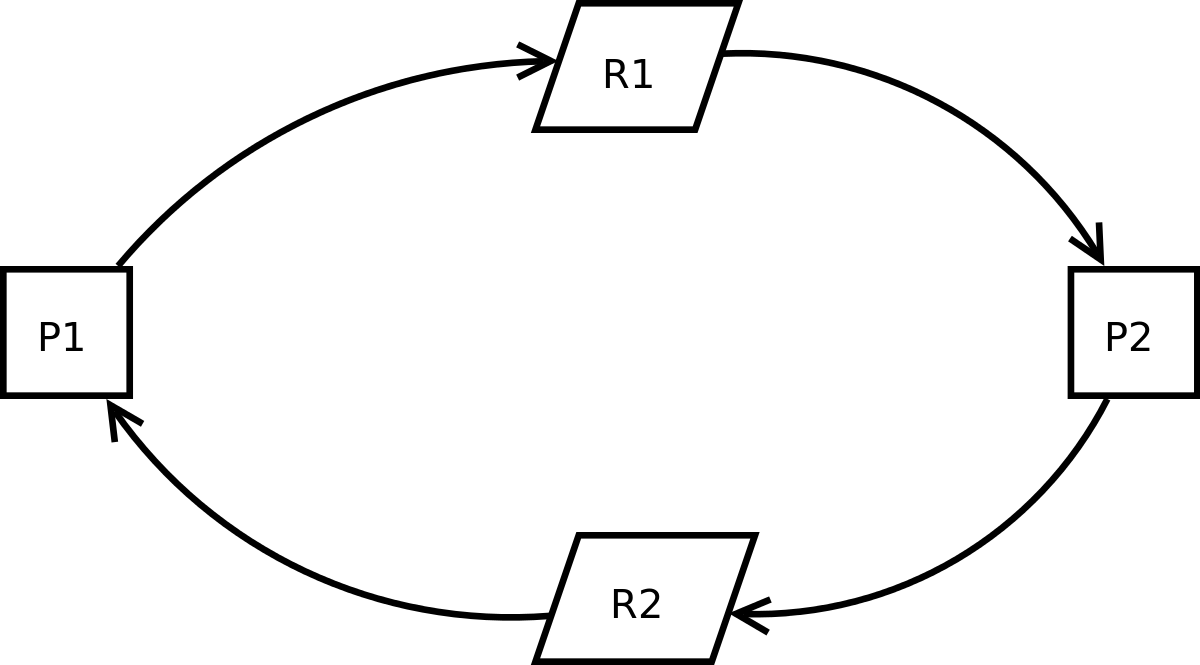
\includegraphics[scale=0.2]{deadlock}
  \centering
  \caption{Exemple d'interblocage}
  \centering
\end{figure}

Souvent pour les programmes avec plusieurs processus et plusieurs ressources, il est difficile de contrôler l'absence d'interblocages, surtout avec la liberté et puissance offertes par la synchronisation.
D'où l'intérêt de reconnaître ces interblocages automatiquement le plus tôt possible, à savoir, éventuellement, lors de la compilation du programme.

\newpage
%%%%%%%%%%%%%%%%%%%%%%%%%%%%%%%%%%%%%%%%%%%%%%%%%%%%
\subsection{Problème et objectifs}

Est-il possible de définir un interblocage pendant l'étape de compilation?\\

 Pour répondre à cette question, l'idée est de commencer par créer une version simplifiée d'un langage parallèle en prenant un langage X10 comme un exemple.
 Le compilateur doit reconnaître juste les instructions qu'on a besoin pour créer plusieurs activités parallèles (boucles, conditions, création de nouveaux processus et horloges).\\
 L'exemple de tel programme est représenté par la Figure 2.

 \begin{figure}[h]
  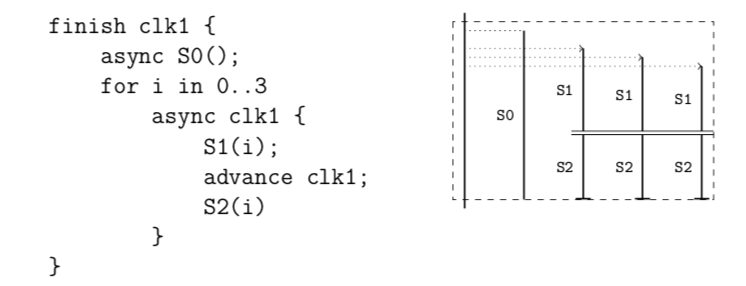
\includegraphics[scale=1]{program}
  \centering
  \caption{Exemple d'un programme parallèle}
  \centering
\end{figure}

 Après avoir implémenté un langage qui permet de créer plusieurs activités parallèles avec la synchronisation, il doit être possible de visualiser l'état de toutes les activités au moment d'interblocages.
 Pour cela, il faut créer une machine virtuelle qui va être capable de simuler l'exécution de programmes parallèles et donner une liste d'activités. \\

 \newpage

 %%%%%%%%%%%%%%%%%%%%%%%%%%%%%%%%%%%%%%%%%%%%%%%%%%%%
 \section{Choix d'implémentation et différentes étapes de réalisation du projet}
 %%%%%%%%%%%%%%%%%%%%%%%%%%%%%%%%%%%%%%%%%%%%%%%%%%%%
Ci-dessous je vais décrire les principales parties de mon travail et préciser le choix d'implémentation. 
% \section{La liste des tâches déjà effectuées}

% \subsection{Le travail réalisé}
% \begin{itemize}
%  \item Installation de librairies et IDE pour le langage de programmation \textbf{X10} sur mon ordinateur.\\ Premièrement, il fallait préparer l'environnement de travail.
%  \item Lecture de la documentation et d'autres ressources sur l'interblocage et programmes parallèles.
%  \item Exécution de différents programmes test X10 pour comprendre le problème et voir comment il fonctionne. 
%  \item Implementation d'un compilateur inspiré par le langage X10 à l'aide de Lexer et parser (Lex et Yacc).
%  \item Génération d'un arbre de la syntaxe abstraite (AST en anglais).
% \end{itemize}


% %%%%%%%%%%%%%%%%%%%%%%%%%%%%%%%%%%%%%%%%%%%%%%%%%%%%
% \section{Le planning prévisionnel des tâches à réaliser}
% \begin{description}
%   \item[mars] Implémentation de la simulation d'exécution du programme et captures de traces d'exécution.
%   \item[avril] Implémentation de visualisation des traces d'execution ou de systèmes mathématiques permettant de détecter un interblocage.
%   \item[mai] Rédiger un rapport avec le bilan de résultats atteints.
% \end{description}

%%%%%%%%%%%%%%%%%%%%%%%%%%%%%%%%%%%%%%%%%%%%%%%%%%%%
\subsection{Le langage}
%%%%%%%%%%%%%%%%%%%%%%%%%%%%%%%%%%%%%%%%%%%%%%%%%%%%

Le langage expérimental dont on a besoin est une version simplifiée (avec les instructions de base)
  d'un langage parallèle de programmation. 
Sa syntaxe se ressemble à celui du langage parallèle X10, un exemple du programme est représenté sur la Figure 3. \\\\Voici les instructions principales du langages dont on a besoin dans le cadre de cette recherche: \\


 \begin{description}[itemsep=2em]
  \item[Boucles et Tests] :

  Pour avoir une possibilité de créer plusieurs activités, le langage doit savoir reconnaître les boucles et vérifier 
  les conditions. \\ Les seules variables dans ce langage sont les compteurs de boucles. \\La syntaxe est la suivante: 


  \begin{itemize} 
    \item \textbf{for i = 0 .. 8 {}} - répéter une instruction pour i de 0 à 8
    \item \textbf{if (i < 7) {}}
  \end{itemize} 


\item[Les instructions de programmation parallèle] :

\begin{itemize} 
  \item \textbf{finish (clock1, ...) {}} - créer un block avec les horloges qu'on peut utiliser pour synchroniser les activités
  \item \textbf{async (clock1, ...) {}} - créer une activité qui peut dépendre d'une clock (p.e. clock1 ici)
  \item \textbf{advance clock1} - créer une barrière de synchronisation sur une clock (clock1 ici)
\end{itemize} 
\newpage
\item[Les horloges] :
 

Chaque instruction peut contenir une horloge (une clock), car c'est un point important dans la programmation parallèle. Les activités sont
indépendantes mais peuvent être enregistrées avec une ou plusieurs horloges communes.\\\\
Les horloges créées par \textit{finish} peuvent être utilisées que à l'intérieur de ce bloc. Pour utiliser une horloge dans une nouvelle activité, 
elle doit être précisée par \textit{async}, cela peut être également une liste de clocks. \\Une barrière de synchronisation \textit{advance} peut utiliser une clock à la fois.\\\\
Il est important de mentionner qu'à tout moment du programme on sait exactement quelles sont les clocks visibles.
\item[les instructions] : 
 
Les instructions ne sont pas importantes dans la recherche, c'est pourquoi seulement les instructions basiques, comme 'S2;', sont présentes.
\end{description}



\begin{figure}[h]
  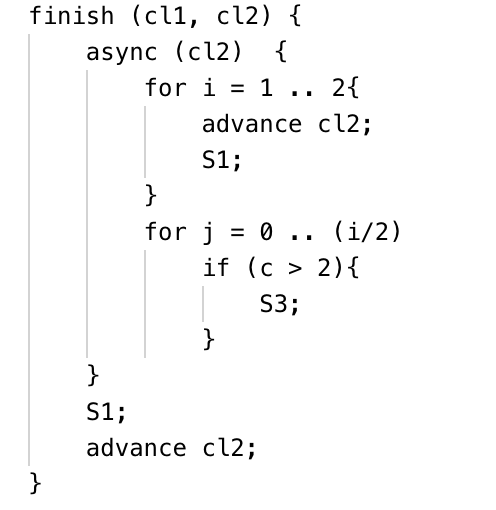
\includegraphics[scale=1]{ex_lang}
  \centering
  \caption{Exemple d'un programme parallèle}
  \centering
\end{figure}

\newpage

%%%%%%%%%%%%%%%%%%%%%%%%%%%%%%%%%%%%%%%%%%%%%%%%%%%%
\subsection{Le compilateur}
%%%%%%%%%%%%%%%%%%%%%%%%%%%%%%%%%%%%%%%%%%%%%%%%%%%%
Les trois parties importantes de la compilation ce sont: un analyseur lexical, un analyseur syntaxique,
 qui produit en sortie un arbre syntaxique abstrait, et un générateur de code intermédiaire.

\subsection{Grammaire}
\begin{lstlisting}
  program -> list_stmt
  stmt -> instruction ';' 
          |   FOR ID '=' range block 
          |   IF '(' affine ')' block  
          |   IF '(' affine ')' block ELSE block
          |   FINISH '(' clocks ')' block
          |   FINISH block
          |   ASYNC '(' clocks ')' block
          |   ASYNC block
          |   ADVANCE ID ';'

  list_stmt -> list_stmt stmt | stmt
  instruction -> ID
  clocks -> clocks ',' ID
          |  ID
          |  eps
  block -> '{' list_stmt '}'
          |   stmt
  range -> affine RANGE affine
  affine -> affine '+' affine
    |   affine '-' affine
    |   affine '/' affine
    |   affine '*' affine
    |   affine COMP affine
    | '(' affine ')'
    | ID
    | NUMBER
\end{lstlisting}
%%%%%%%%%%%%%%%%%%%%%%%%%%%%%%%%%%%%%%%%%%%%%%%%%%%%
\newpage

\subsection{Construction d'un arbre syntaxique abstrait}
L'analyseur syntaxique produit comme résultat un arbre syntaxique abstrait, un AST à la suite, 
qui est utilisé plus tard pour effectuer une analyse sémantique et générer de code intermédiaire.

La structure d'un AST contient 12 types de nœuds - un nœud par instruction  : 
\begin{itemize} 
  \item id
  \item number
  \item basic
  \item advance
  \item finish
  \item async
  \item operation
  \item assignment
  \item for 
  \item range
  \item statements
  \item if
\end{itemize}

Chaque nœud peut avoir au maximum trois fils. \\\\ Il est possible de visualiser un arbre syntaxique abstrait généré grâce à une fonction \textit{ast\_print(ast,indent)}. 
\\\\Le résultat est présenté sur la Figure \ref{fig:ast} où on peut remarquer que l'hiérarchie de l'arbre est obtenue à l'aide d'indentation.
%+ exemple
\begin{figure}[h]
  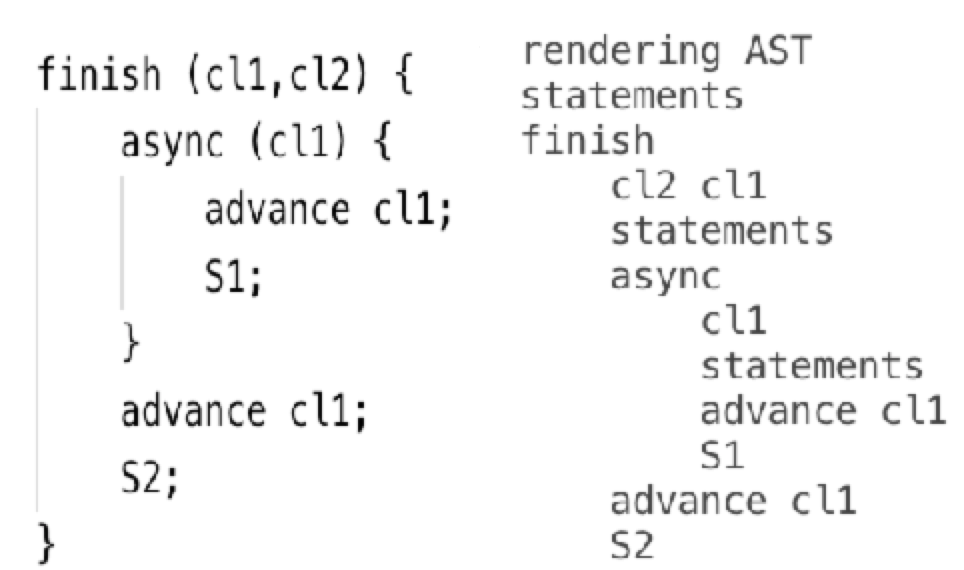
\includegraphics[scale=0.5]{ast_exemple}
  \centering
  \caption{Exemple d'un résultat de la fonction \textit{ast\_print(ast,indent)}}
  \centering
  \label{fig:ast}
\end{figure}

\newpage

\subsection{Vérification sémantique}
Après construire un arbre, les vérifications sur la sémantique du programme sont effectuées. 

L'analyse sémantique comprend: 


\begin{description}
  \item[une détection de l'utilisation de variables non initialisées] - comme dans le langage les seules variables sont les compteurs de boucles, il ne peuvent pas être utilisés avant cette boucle.
  \item[une détection des horloges utilisées en dehors de leur portée] - l'activité n'est pas inscrite à une clock ne peut pas l'utiliser.
\end{description}

L'analyseur sémantique parcours récursivement un AST et compare les variables et les horloges rencontrées avec le contenu de la table de symboles.\\
Une clock est supprimée de la table de symboles à chaque fois quand elle est en dehors de la portée d'une instruction. De cette façon, l'instruction comme async ou advance ne peut pas utiliser 
une horloge qui n'est pas visible pour elle.




%%%%%%%%%%%%%%%%%%%%%%%%%%%%%%%%%%%%%%%%%%%%%%%%%%%%
\subsection{Machine virtuelle}
%%%%%%%%%%%%%%%%%%%%%%%%%%%%%%%%%%%%%%%%%%%%%%%%%%%%
Ayant un langage avec les instructions parallèles, il est possible de choisir entre une machine virtuelle parallèle 
et une machine virtuelle séquentielle pour simuler l'exécution du programme. \\\\ Etant donné que le but principal de l'interpréteur est de pouvoir produire la liste des
activités en cours et pas la performance du programme, j'ai décidé d'utiliser un principe de l'exécution séquentielle. 
Cela veut dire, que seulement une activité est exécutée à la fois. 

Ainsi, la machine virtuelle l'exécutera chaque activité \textbf{pas à pas} jusqu'au moment qu'elle sera bloquée et seulement après cela 
la prochaine activité dans une pile va s'exécuter.

\newpage
\subsection{Les structures de données de la machine virtuelle}

Pour capturer des traces d'exécutions, on garde l'information principale sur un programme,
telle que toutes les clocks créées, toutes les activités inscrites avec ces clocks etc.

Voici la structure de la machine virtuelle: \\

\begin{description}
  \item[state] : 
   
  \begin{itemize} 
    \item \textbf{ready} - une liste d'activités prêtes à être exécutées
    \item \textbf{running} - une activité en cours d'exécution
  \end{itemize} 

  \item[activity] : 
   
  \begin{itemize} 
    \item \textbf{id} - l'identifiant d'une activité
    \item \textbf{program counter} - le compteur ordinal, que l'activité incrémente après la lecture d'une instruction et les instructions de saut écrivent dedans.
    \item \textbf{finish stack} - une pile de pointeurs sur les structures de finish englobants
    \item \textbf{registered with} - une liste d'horloges avec lesquelles l'activité est enregistrée
  \end{itemize} 

  \item[finish] : 
   
    \begin{itemize} 
       \item \textbf{id} - l'identifiant d'un finish
       \item \textbf{clocks} - les horloges créées par ce finish
       \item \textbf{activities} - les activités qui sont dans le bloc du finish
       \item \textbf{is waiting} - un flag qui indique si ce finish est en attente de la terminaison de ces activités
    \end{itemize} 

  \item[clocks] : 
    
    \begin{itemize} 
      \item \textbf{id} - l'identifiant d'un clock
      \item \textbf{registered} - la pile d'activités enregistrées avec ce clock
      \item \textbf{blocked} - la pile d'activités bloquées par ce clock
    \end{itemize} 

\end{description}

\newpage

\subsection{L'exécution du code intermédiaire}
%%%%%%%%%%%%%%%%%%%%%%%%%%%%%%%%%%%%%%%%%%%%%%%%%%%%
% expliquer pq on a choisi code -> exec au lieu de ast -> exec
\noindent Le code intermédiaire est généré à partir d'un arbre de syntaxe abstrait. \\\\
Il est possible d'exécuter directement un AST sans générer le code, mais 
comme la machine virtuelle pas à pas a besoin de pouvoir retourner en arrière quand elle 
fait une boucle ou un changement d'activité, c'est plus logique d'avoir le code avec un compteur ordinal
que garder un chemin de l'arbre pour chaque instruction. \\\\
Ci-dissous une spécification sur l'exécution des instructions principales de programme.\\


\begin{description}

  \item[FINISH] : 
  \begin{itemize} 
    \item créer une nouvelle structure finish
    \item la rajouter dans une pile de finish de l'activité en cours
  \end{itemize} 

  \item[CLOCK CREATE] : 
    \begin{itemize} 
       \item créer une nouvelle structure clock
       \item ajouter l'activité en cours dans la pile 'registered' enregistrées avec ce clock
       \item ajouter ce clock dans une pile de clocks de l'activité en cours
       \item rajouter ce clock dans une pile de clocks de finish de l'activité en cours
    \end{itemize} 

  \item[END FINISH] : 
    
    si la pile d'activités créées dans ce finish n'est pas vide, alors : 
    \begin{itemize} 
      \item mettre l'état 'is waiting' de finish à vrai
      \item pour chaque clock créée par ce finish enlever l'activité en cours de la pile 'registered' de ce clock
      \item enlever l'activité en cours de la pile d'activités prêtes à être exécutées
    \end{itemize} 
    sinon mettre l'état de finish 'is waiting' à faux et détruire les clocks créés par ce finish

  \item[ASYNC] : 
    \begin{itemize} 
      \item créer une nouvelle activité avec le compteur du programme égal à label suivant et le finish englobant dans la pile de finish
      \item ajouter cette activité dans 'ready' et dans une pile d'activités créées par le finish
    \end{itemize} 
  
   \item[CLOCK REGISTER]:
    \begin{itemize} 
      \item rajouter le clock dans une pile de clocks de l'activité en cours
      \item ajouter l'activité en cours dans la pile 'registered' de ce clock
    \end{itemize} 

   \item [END ASYNC] :
    \begin{itemize} 
      \item enlever l'activité en cours de la pile 'registered' pour tous les clocks avec lesquels elle était enregistrée
      \item enlever l'activité en cours de la pile d'activités du finish englobant
      \item enlever l'activité en cours de la liste 'ready'
    \end{itemize} 

   \item [ADVANCE] :
    \begin{itemize} 
      \item rajouter l'activité en cours dans la pile 'blocked' du clock
      \item enlever l'activité en cours de la liste 'ready'
      \item si les piles 'blocked' et 'registered' du clock sont identiques, 
      déplacer les activités qui étaient dans la pile 'blocked' dans la liste 'ready'
    \end{itemize} 

\end{description}



\subsection{Evaluation des expressions arithmétiques}
L'évaluation des expressions arithmétiques s'effectue à l'aide d'une pile. Plus précisément, on mets les résultats intermédiaires
dans la pile et la manipule pour faire le calcul. 
Si le programme a plusieurs variables (plusieurs compteurs de boucles) leurs valeurs sont stockés sur les positions concrètes 
de la pile (sous les premiers indices) et sont mis à jour à chaque itération. 

Sur la Figure \ref{fig:pile} on peut observer une schéma qui montre le principe du calcul. 

\begin{figure}[h]
  \subfloat[]{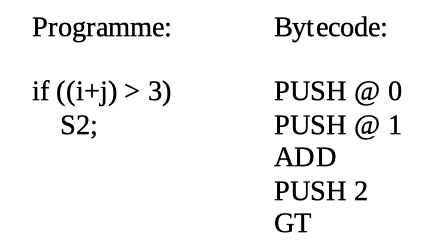
\includegraphics[scale=0.8]{prog_pile}}
  \subfloat[]{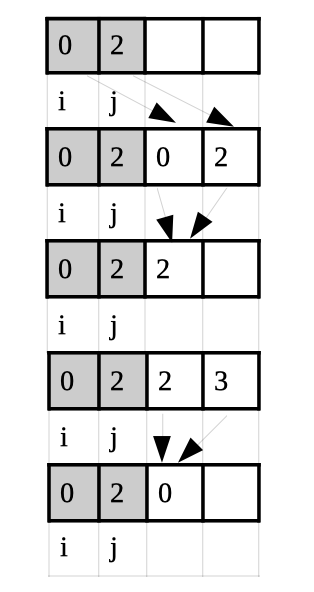
\includegraphics[scale=0.5]{pile}}
  \centering
  \caption{Exemple d'évaluation des expressions à l'aide de la pile}
  \centering
  \label{fig:pile}
\end{figure}

\newpage 
Pour exécuter ces expressions les instructions spéciales sont présentes dans le code intermédiaire, 
telles que les instructions:


\begin{itemize} 
  \item \textbf{PUSH @ 0} - ajouter une nouvelle variable à l'adresse 0 de la pile
  \item \textbf{PUSH 3} - empiler un entier 3
  \item \textbf{ADD, MULT, DIV, SUB} - effectuer une opération affine entre les deux valeurs qu'ils sont dans la pile
  \item \textbf{LT, GT, EQ, NE,\dots} - effectuer un comparaison entre les deux valeurs qu'ils sont dans la pile
\end{itemize} 


Le principe de l'évaluation à l'aide de la pile est assez simple et n'est pas en priorité pour ce recherche, c'est pourquoi 
seulement le code intermédiaire pour les expressions arithmétiques est implémenté dans la version courante du projet.



%%%%%%%%%%%%%%%%%%%%%%%%%%%%%%%%%%%%%%%%%%%%%%%%%%%%
\section{Conclusion}
%%%%%%%%%%%%%%%%%%%%%%%%%%%%%%%%%%%%%%%%%%%%%%%%%%%%
Le but de mon travail d'étude et de recherche était de simuler l'exécution de programmes parallèles et d'avoir la possibilité
de détecter l'interblocage. Dans son cadre un langage de programmation parallèle a été créé basé sur le langage déjà existant X10
mais seulement avec les instructions nécessaires pour la suite de la recherche. 

Pour cela l'analyseur lexical et l'analyseur syntaxique étaient implémentés avec comme résultat un arbre de syntaxe abstrait. 
Le code intermédiaire est généré en parcourant un AST. La machine virtuelle séquentielle réalisée, parcours pas à pas ce code intermédiaire
et est capable d'afficher l'état global de chaque activité avec l'état d'horloges créées.

Grâce à ce travail il est possible maintenant de détecter un interblocage et analyser l'état de la machine virtuelle pour savoir les horloges et les activités 
qui ont provoqué cet interblocage.

Pour aller plus loin, on pourrait faire une visualisation interactive de l'état d'exécution d'un programme parallèle.

\newpage      
%%%%%%%%%%%%%%%%%%%%%%%%%%%%%%%%%%%%%%%%%%%%%%%%%%%%
\begin{thebibliography}{9}
  \bibitem{sujet} 
  Alain Ketterlin.
  \textit{La présentation de sujet de TER}. 
   
  \bibitem{parallel} 
  Agarwal Shivali, Barik Rajkishore, Sarkar Vivek, Shyamasundar R.K.\\
  \textit{May-happen-in-parallel analysis of X10 programs}.
  Proceedings of the ACM SIGPLAN Symposium on Principles and Practice of Parallel Programming (2007), PPOPP.
   
  \bibitem{x10} 
  Vijay Saraswat, Bard Bloom, Igor Peshansky, Olivier Tardieu, and David Grove
  \textit{X10 Language Specification}. 
  Version 2.6.2

  \bibitem{deadlock} 
  Composing Programs: Parallel Computing,
  \\\texttt{https://composingprograms.com/pages/48-parallel-computing.html}
  \end{thebibliography}
 \addcontentsline{toc}{section}{Références}
 \bibliographystyle{alpha}

\end{document} 
%%%%%%%%%%%%%%%%%%%%%%%%%%%%%%%%%%%%%%%%%%%%%%%%%%%%
